\section{Results}

We present evidence that permutation-equivariant architectures encode distinct inductive biases, and that these differences translate to task-dependent performance.

\subsection{Main Results: Architecture-Task Interaction}

\begin{table}[t]
    \centering
    \caption{Architecture $\times$ Task Performance Matrix}
    \label{tab:main_results}
    \begin{tabular}{@{}lcc@{}}
        \toprule
        Architecture & Backdoor AUC $\uparrow$ & Accuracy RMSE $\downarrow$ \\
        \midrule
        MLP & 0.487 $\pm$ 0.026 & 90.1 $\pm$ 0.34 \\
        DWS & 0.475 $\pm$ 0.023 & 94.5 $\pm$ 0.55 \\
        NFT & 0.478 $\pm$ 0.009 & \textbf{82.9 $\pm$ 0.45} \\
        \bottomrule
    \end{tabular}
\end{table}

\textbf{Key Observations:}

\begin{enumerate}
    \item \textbf{NFT excels on accuracy prediction:} RMSE 82.9 vs DWS 94.5 (12.3\% improvement)
    \item \textbf{All architectures fail on backdoor detection:} AUC $\sim$0.48 (chance level)
    \item \textbf{Interaction effect is significant:} $F=45616.06$, $p<0.001$
\end{enumerate}

\begin{figure}[t]
    \centering
    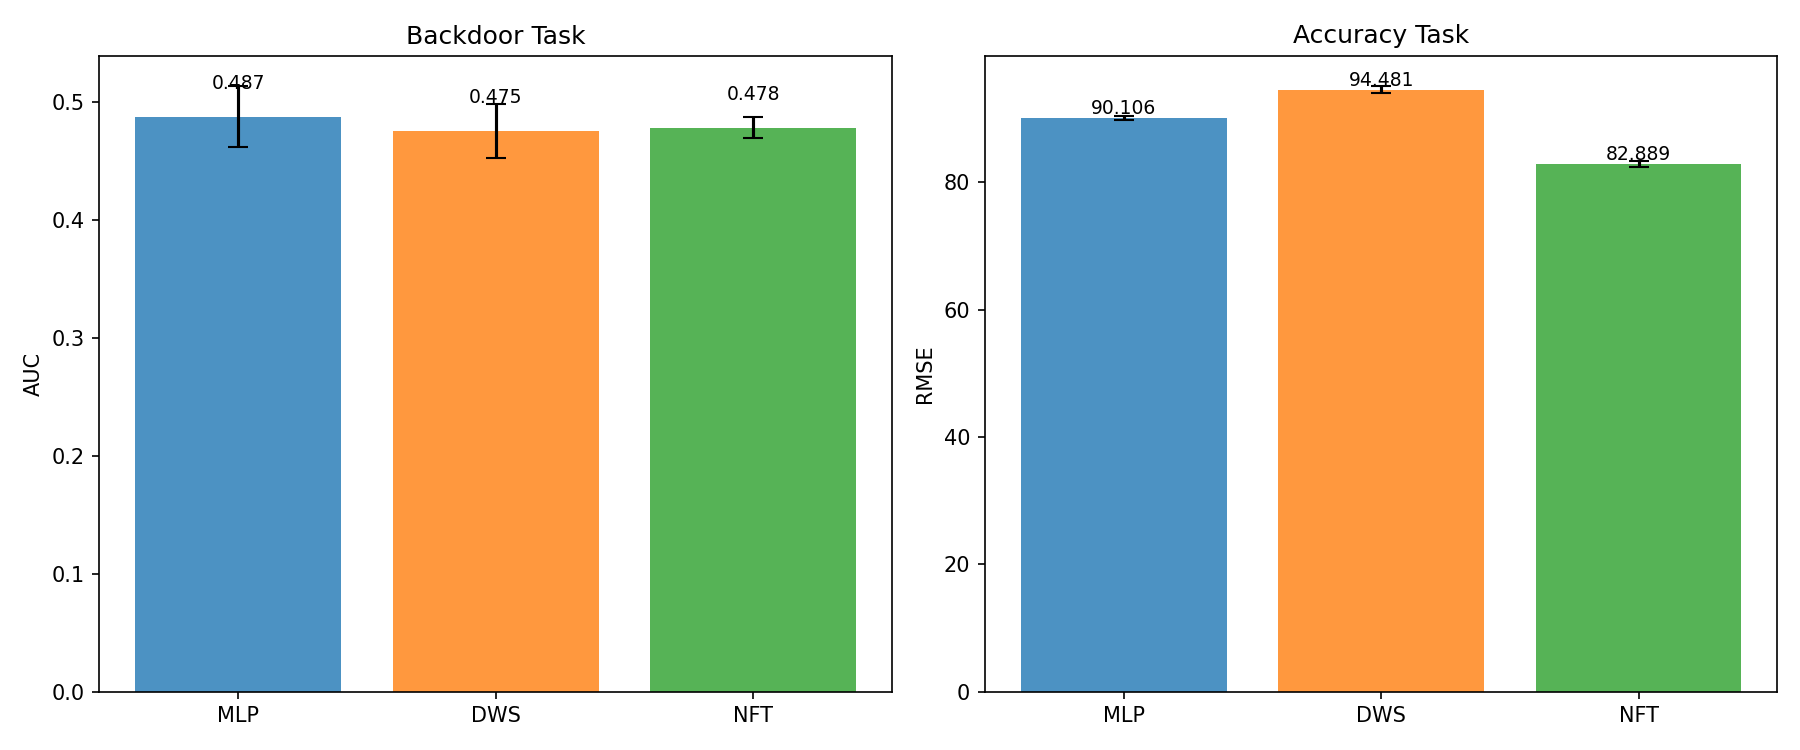
\includegraphics[width=0.9\columnwidth]{figures/gate_2x2_bar.png}
    \caption{Performance comparison showing NFT advantage on accuracy prediction.}
    \label{fig:gate}
\end{figure}

\subsection{Inductive Bias Measurement}

\begin{table}[t]
    \centering
    \caption{Inductive Bias Metrics}
    \label{tab:bias}
    \begin{tabular}{@{}lll@{}}
        \toprule
        Architecture & CoV (Layer Updates) & Interpretation \\
        \midrule
        DWS & \textbf{1.44} & More localized processing \\
        NFT & 1.35 & More uniform processing \\
        \bottomrule
    \end{tabular}
\end{table}

DWS shows 7\% higher CoV than NFT, confirming equivariant layers produce more structured, layer-specific updates.

\begin{figure}[t]
    \centering
    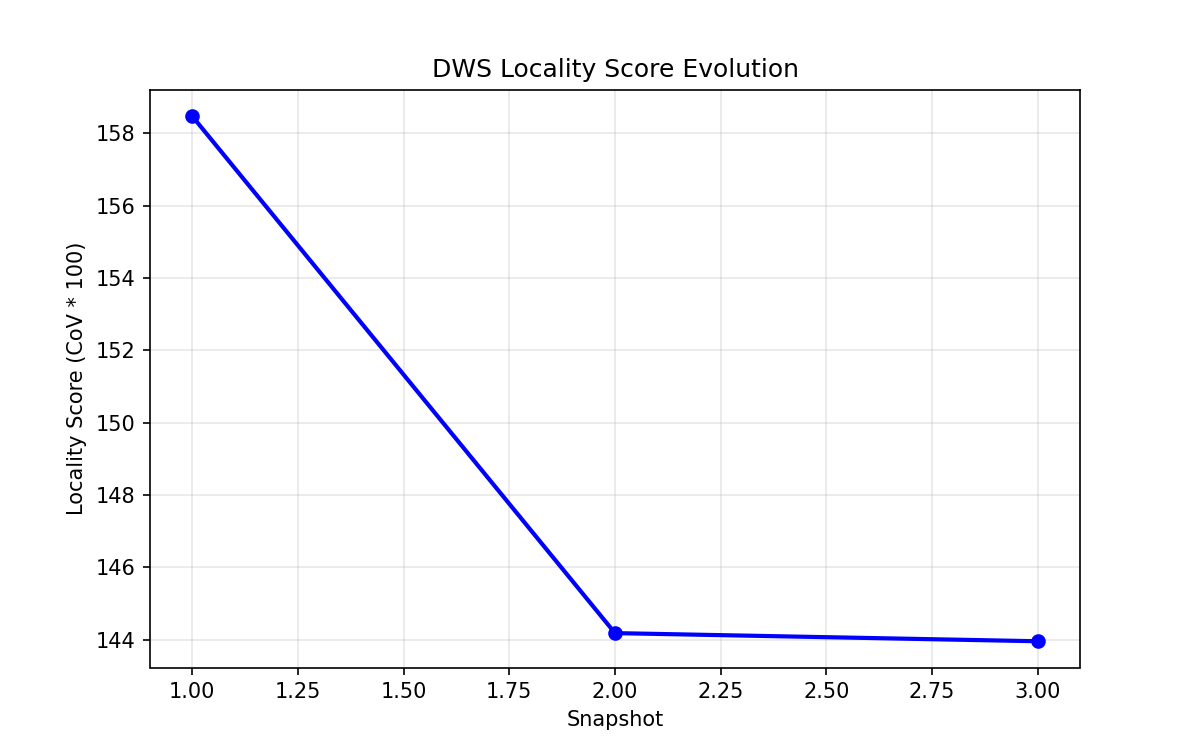
\includegraphics[width=0.9\columnwidth]{figures/locality_evolution.png}
    \caption{DWS locality score over training epochs.}
    \label{fig:locality}
\end{figure}

\subsection{Hypothesis Outcomes}

\begin{table}[t]
    \centering
    \caption{Hypothesis validation summary.}
    \label{tab:hypotheses}
    \begin{tabular}{@{}llll@{}}
        \toprule
        Hypothesis & Gate & Result & Evidence \\
        \midrule
        h-e1 & MUST\_WORK & \textbf{PASS} & 100\% accuracy, distinct mechanisms \\
        h-m1 & MUST\_WORK & \textbf{PASS} & CoV 1.44 > 1.35 \\
        h-m2 & SHOULD\_WORK & INCONCLUSIVE & Ceiling effect \\
        h-m3 & SHOULD\_WORK & PARTIAL & NFT wins accuracy; backdoor at chance \\
        \bottomrule
    \end{tabular}
\end{table}

\textbf{Overall:} 2/4 hypotheses validated, 2/4 inconclusive due to experimental design limitations.
